\appendix
\onecolumn


\section{The UCL Vision Research Lab's expression space pipeline}
\label{a:pipeline}
This section describes how a single still face-image (and, by extension, a video formed of a sequence of images) can be represented as a series of coefficients which (together with a specially defined ``face space") can reproduce a given face-image with a high degree of accuracy and a great deal of compression; a face-image can be specified by the coefficients alone (provided the face space is already given), information which is orders of magnitude smaller than the bitmapped version of the image.

Heavy use is made of the technique of \textit{principal component analysis} or \textit{PCA}\cite{wood1987principal}\footnote{Also known as the discrete Karhunen-Lo\`eve transform, the Hotelling transform or proper orthogonal decomposition.}, a technique which highlights the axes of largest variance in a set of multivariate point data. Consider an $d$-dimensional space containing $n$ points. Each point is defined by $d$ coordinates along the normal axes of the space. PCA imposes $b$ \textit{new axes} on the space (the choice of $b$ is down to the operator, subject to $b<d$) and expresses each point by $b$ coordinates along each of these new axes.

Each new axis is chosen so that it spans the maximum possible variance among the points, given the important constraint that the new axes (like the old ones) must be orthonormal. For example, imagine a data set which looks like a vaguely cylindrical point cloud in the original $d$-space. The axis of greatest variance will be along the longditudinal axis of the point cloud; this, therefore, will be the first axis of $b$-space. See figure \ref{f:spaces} for an illustration. Mathematically, the transformation can be done by finding the eigenvectors and eigenvalues of the covariance matrix of the initial variables.

After PCA each point is described by a $b$-vector, along with the origins and directions of the $b$ new axes (which are the same for every point and must therefore only be given once for the data set).  If $b=d$, PCA merely rotates the data set and every point is still described fully; information is not lost. If $b<d$, some information about the precise location in $d$-space of each point is lost. The larger $b$, the smaller the information loss and the smaller the compression. PCA is therefore user-parametrisable in terms of $b$, allowing an adjustable tradeoff between compression and accuracy.

The first research on the application of PCA to faces was done by Sirovich \etal in 1987\cite{sirovich1987low}, who evaluated the feasibility of the technique on a set of example faces. Taking each face (a 128 $\times$ 128 pixel greyscale picture) as a point in $D$-dimensional space, with $D= 128^2 = 2^{14}$, they performed PCA to extract a series of $B$ basis vectors spanning the subspace in which the example faces were situated. They noted that each face can be expressed
%CHECK THIS
by adding together a series of ``eigenfaces" (points in $B$-space, each one generated by extending a basis vector by a certain coefficient). To make their method work, Sirovich \etal had to perform a substantial degree of cropping and normalisation before applying PCA; their test set was also composed exclusively of young Caucasian males.

A major problem with feeding a linearised image directly into the PCA procedure, then linearly combining eigenfaces into an output face, is that linear combinations produce inherent blur; combining two widely differing eigenfaces will not produce a realistic-looking face but a blurred combination of the two. This is a reflection of the fact that faces are not pure mathematical artefacts but physiological objects whose shape is constrained by their underlying musculoskeletal structure.

Work over the intervening years has extended this simplistic application of PCA into a more mature method capable of dealing with a wider variety of faces and expressions in full colour. The following procedure is typical of the processing pipeline used by the UCL Vision Research Lab.

To take into account shape information as well as texture information, all frames are first conceptually shape-standardised using a warping operation\footnote{\textit{Warping} simply spatially deforms an image; \textit{morphing} combines spatial deformation with blurring between a start and finish image.} The input to the PCA process consists of \textit{a)} RGB or greyscale pixel data specifying a base image, and \textit{b} a vector flow field allowing this base image to be warped into a final output image. This separates texture data from shape data (even though this division is to some degree arbitrary, as discussed later). 

The input to the procedure is a sequence of frames $f_i$ and a reference frame $A$ (selected so as to contain colour components allowing realistic warping to a large amount of expressions, such as an open mouth showing teeth and a dark area between the teeth. Warping can remove colours from an image by reducing their area to zero, but not add them).

\begin{enoomerate}
\item Using the multichannel gradient model (MCGM) algorithm\cite{mcowan1995algorithms}, a neurally plausible motion-detection and warp-finding algorithm, generate warp fields $W_i$ from each $A$ to each $f_i$. Each warp field is simply a vector field showing how to deform $A$ to obtain $f_i$.

\begin{center}
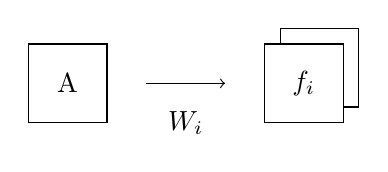
\begin{tikzpicture} 
\draw (1,1) +(-.5,-.5) rectangle ++(.5,.5); \draw (1,1) node{A};
\draw (4,1) +(-.3,-.3) rectangle ++(.7,.7); \draw (4,1) node{$f_i$};
\draw[fill=white] (4,1) +(-.5,-.5) rectangle ++(.5,.5); \draw (4,1) node{$f_i$};
\draw (2.5,0.5) node{$W_i$};
\draw[->] (2,1) -- (3,1);
 \end{tikzpicture}
\end{center}

\item Average these fields, generating a mean warp $W_m$.
\item Warp the reference image with the mean warp to generate the warp mean $M$.

\begin{center}
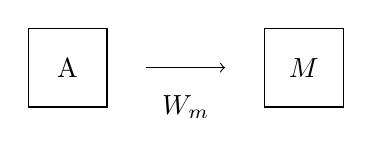
\begin{tikzpicture} 
\draw (1,1) +(-.5,-.5) rectangle ++(.5,.5); \draw (1,1) node{A};
\draw (4,1) node{$f_i$};
\draw[fill=white] (4,1) +(-.5,-.5) rectangle ++(.5,.5); \draw (4,1) node{$M$};
\draw (2.5,0.5) node{$W_m$};
\draw[->] (2,1) -- (3,1);
 \end{tikzpicture}
\end{center}

\item Generate new warp fields $W_i^\prime$ which warp the warp mean to each frame $f_i$ (not to the reference image). These warp fields are generated by taking the reverse of the mean warp, then doing the initial warps $W_i$.
These new fields $W_i^\prime$ each symbolise the warp required to reshape the warp mean into the shape of the face in frame $f_i$.

\begin{center}
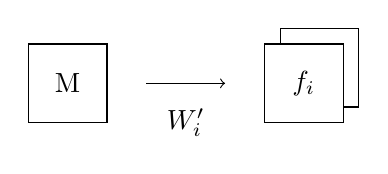
\begin{tikzpicture} 
\draw (1,1) +(-.5,-.5) rectangle ++(.5,.5); \draw (1,1) node{M};
\draw (4,1) +(-.3,-.3) rectangle ++(.7,.7); \draw (4,1) node{$f_i$};
\draw[fill=white] (4,1) +(-.5,-.5) rectangle ++(.5,.5); \draw (4,1) node{$f_i$};
\draw (2.5,0.5) node{$W_i^\prime$};
\draw[->] (2,1) -- (3,1);
 \end{tikzpicture}
\end{center}

\item Apply the reverse warps of fields $W_i^\prime$ to each frame. This results in a set of frames $f_i^\prime$ which all have the \textit{shape} of the warp mean, but different texture information.
\item For each frame, store $f_i^\prime$ and $W_i^\prime$. Each original frame can be reconstructed by applying $W_i^\prime$ to $f_i^\prime$.
\item Serialise this information (by concatenating the lists ${r_i,g_i,b_i,x_i,y_i}$ containing red, green, blue and ${x,y}$-warp information for each pixel) for each frame. Each frame is now symbolised by a high-dimensional vector containing colour and warp information; these vectors exist in an $f$-dimensional \textit{frame space}. Frame space, of course, contains all possible images, including those which do not represent faces.
\item Perform PCA on the resulting point cloud. The space spanned by the $e$ principal components chosen is an $e$-dimensional \textit{expression space}; each point therein represents an expression.
\item Reconstruct expressions by taking a point in $e$-space (either representing a real expression, or an artificial one), projecting it into frame space, warping its image data with its warp data, and displaying it.
\end{enoomerate}

This process is summarised in figure \ref{f:spaces}.


\section{Source code}
\label{appb}

The following pages show Matlab source code for the two main functions of the report: building a second-order PCA space and reclaiming a video therefrom. Much functionality is included in external functions.

\cleardoublepage

\section{Video files}
\label{appc}

The included CD contains video files showing various comparative reconstructions generated during the experiment.


\begin{itemise}
\item One clip reconstructed with different values of $s$.
\item Side-by-side comparisons of original and reconstructed clips, $s$=7.
\item Some random dynamic expressions, $s$=7.
\item Comparison of the clips produced in section \ref{stddevs} showing the effect of increasing or decreasing each principal component.
\end{itemise}
\cleardoublepage

\section{Jokes used to generate the smiles during filming}
\label{appa}

\begin{itemise}
\item What did the ham say to the doctor?\\
\textit{I'm cured!}
\item Why did Bambi start smoking?\\
\textit{Deer pressure!}
\item Why did Little Jack Horner sit in the corner?\\
\textit{Because his bum was square.}


\item Why was the electron depressed?\\
\textit{It felt a bit negative.}


\item A horse walks into a bar. ``Why the long face?" the barman says. ``My wife has left me and I'm an alcoholic," says the horse.


\item A hole has been found in a naturist camp wall. The police are looking into it.

\item What do you call a man with seagulls nesting in his head?\\
\textit{Cliff!}


\item What do you call a man with rabbits burrowing into his head?\\
\textit{Warren.}


\item Some trees were stolen from my local forest. The police are stumped.

\item Later the same day, all the toilet seats were stolen from my local police station. The police have nothing to go on.

\item On the news today... police were called to my local nursery school where a two-year-old was resisting a rest.


\item When Prince William joined the army he disliked the use of the phrase ``Fire at Will!"


\item We have a saying where I come from. Time flies like an arrow. Fruit flies like a banana.


\item What's a prisoner's favourite punctuation mark?\\
\textit{The full stop. It marks the end of his sentence.}


\item Did you hear about the soldier who survived attacks of mustard gas and pepper spray? He was a seasoned veteran.


\item When is a door not a door?\\
\textit{When it's a jar.}

\item When is a car not a car?\\
\textit{When it turns into a side street.}

\item Did you hear about the short fortune-teller who escaped from prison? He was a small medium at large.

\item The Energizer bunny was arrested for being violent. He was charged with battery.

\item Have you heard about the new practice of coffee-stealing? They call it ``mugging."

\item A fire ripped through the campsite. The heat was intense.

\item My friend went on holiday to Egypt, but couldn't accept that he was really there. I think he was in denial.


\item Why do tennis players rarely marry?\\
\textit{Because love means nothing to them.}

\end{itemise}
\end{document}
